\documentclass{article}

\usepackage{graphicx}
\usepackage{amsmath}
\usepackage{amssymb}

\newcommand{\R}{\ensuremath{\mathbb{R}}}

\begin{document}
\section{Approximating a summation}
It is not always possible to find a closed-form expression for a sum. For example, no closed form is known for

$$
S = \sum_{i = 1}^{n} \sqrt{i}
$$

In such cases, we have to resort to approximating sums.

Let $f : \R^{+} \rightarrow \R^{+}$ be a \textit{non decreasing function}. Define

$$
S ::= \sum_{i = 1}^{n}f)i
$$

and

$$
I ::= \int_{1}^{n} f(x).dx
$$

Then

$$
I + f(1) \le S \le I + f(n)
$$

\textit{Similarily}, if $f$ is \textit{non increasing}, then

$$
I + f(n) \le S \le I + f(1)
$$

\paragraph{Proof}
Suppose $f : \R^{+} \rightarrow \R^{+}$ is non decreasing. The value of $S$ is the sum of the areas of $n$ unit-width rectangles of height $f(1), f(2), \dots, f(n)$. The areas are shown in the following figure:

\begin{figure}[h!]
    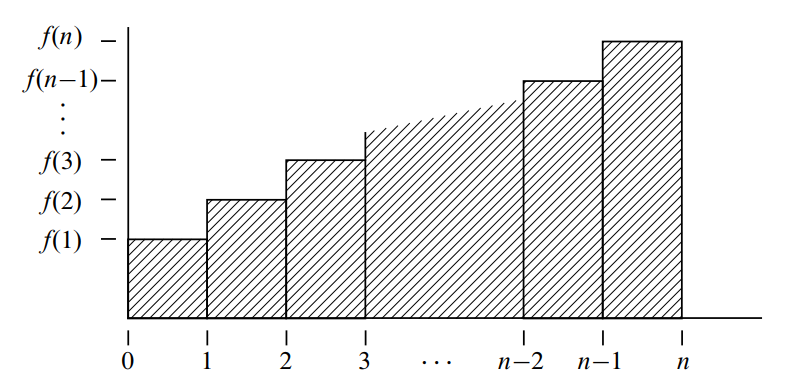
\includegraphics[width=\linewidth]{resources/13_1.png}
    \caption{Figure 1}
    \label{fig:p1}
\end{figure}

The value of $I$ is shown in the figure below:

\begin{figure}[h!]
    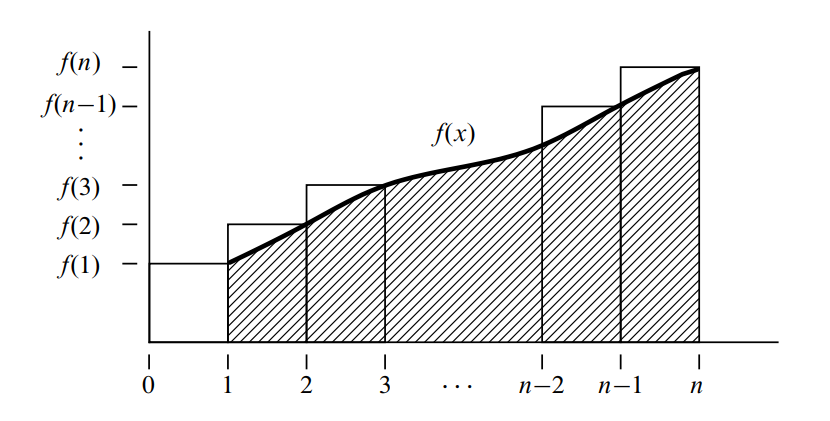
\includegraphics[width=\linewidth]{resources/13_2.png}
    \caption{Figure 2}
    \label{fig:p2}
\end{figure}

Comparing the above two figures, the lower bound of the area can be seen as $f(1) + I$. Therefore, $S \ge f(1) + I$.

To derive the area for the upperbound, we shift the curve to one unit by left as shown below.

\begin{figure}[h!]
    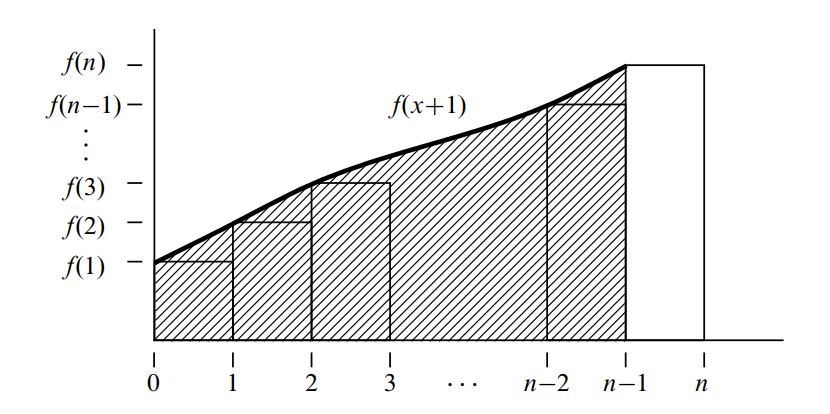
\includegraphics[width=\linewidth]{resources/13_3.png}
    \caption{Figure 3}
    \label{fig:p3}
\end{figure}

Now, the upperbound can be easily seen as $I + f(n)$, Therefore $S \le I + f(n)$. 

A similar analysis can be done for \textit{non increasing functions}, or you can just see that the mirror image of the graph of a \textit{non decreasing function} is a \textit{non increasing function} and replace $x$ with $-x$ to get the mirror image and invert the equality signs.

\section{Asymptotic Notion}

Note: All of these relations are on functions.

\begin{enumerate}
    \item \textbf{Asymptotic Equivalence (\~)}

        Def: $f(n) ~ g(n)$

        $$
            \lim_{n \rightarrow \infty} \frac{f(n)}{g(n)} = 1
        $$

        For example, $n^2$ $n^2 + n$ because

        $$
            \lim_{n \rightarrow \infty} \frac{n^2 + n}{n^2} = 1
        $$

        \~ is an equivalence relation.

    \item \textbf{Asymptotically smaller (Little Oh: o(.))}

        Def: $f(n) = o(g(n))$ iff

        $$
            \lim_{n \rightarrow \infty} \frac{f(n)}{g(n)} = 0
        $$

        o(.) is a strict partial order relation

    \item \textbf{Asymptotic Order of Growth (Big Oh: O(.))}

        Def: $f = O(g)$

        $$
            \limsup_{n \rightarrow \infty} \frac{f(n)}{g(n)} < \infty
        $$

        O(.) is a strict partial order relation

    \item \textbf{Same order of growth ($\theta$)}

        Def: $f = \theta(g)$  

        $$ 
        f = O(g) 
        $$ 
 
        and 
 
        $$ 
        g = O(f) 
        $$ 
  
        $\theta(.)$ is an equivalance realtion

\end{enumerate}

\end{document}
